\subsection{GPIO/UART/I2C/1-Wire/SPI interfaces}
\label{sec:wrpc_periph}

%\begin{figure}[ht]
%  \begin{center}
%    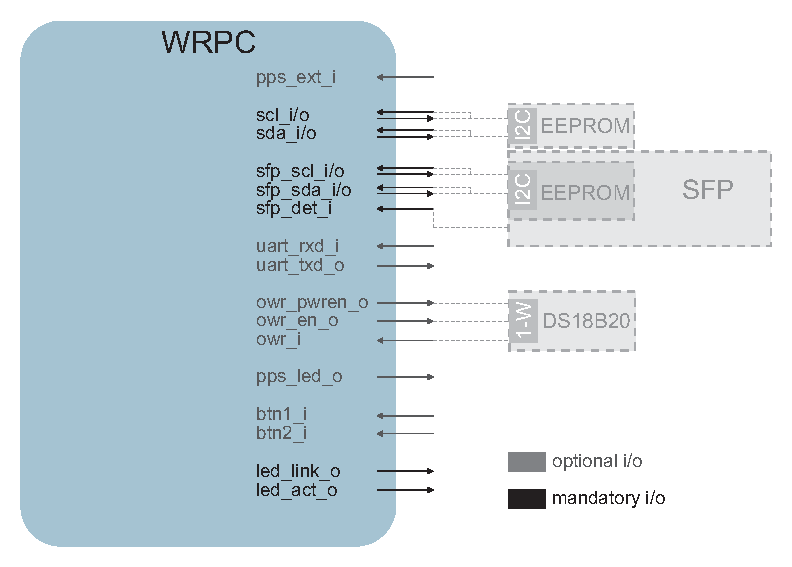
\includegraphics[width=.9\textwidth]{fig/basic_wrpc_gpio.pdf}
%    \caption{Other interfaces of WRPC}
%  \end{center}
%\end{figure}

Several hardware peripherals can be connected to the White Rabbit PTP Core. It
has:
\begin{itemize}
  \item UART - provides access to the WR PTP Core user shell
  \item 1-Wire - access to a digital thermometer for an on-board temperature and
    unique ID (used to generate a default MAC address of the WR port)
  \item SFP $I^2C$ - access to the SFP EEPROM, to read its ID and math with the
    calibration values
  \item SPI - access to the Flash memory, used to store calibration
    parameters and init script
  \item EEPROM $I^2C$ - [optional] access to the EEPROM memory, used to store
    calibration parameters and init script - currently SPI Flash is the
    preferred storage, however, EEPROM can still be used if needed.
\end{itemize}
